\documentclass[11pt,a4paper]{article}

\usepackage{cmap}
\usepackage[T1]{fontenc}
\usepackage[utf8]{inputenc}
\usepackage{natbib}
\usepackage[french,english]{babel}
\frenchsetup{SmallCapsFigTabCaptions=false}
\usepackage{lmodern}
\usepackage{microtype}
\usepackage{geometry}
\usepackage{amsmath,amssymb,mathtools}
\usepackage{booktabs,tabularx,array}
\usepackage{graphicx}
\usepackage{xcolor}
\usepackage{enumitem}
\usepackage{caption}
\usepackage{xurl}
\usepackage[unicode=true,pdfencoding=auto]{hyperref}
\usepackage{fancyhdr}

\geometry{left=24mm,right=24mm,top=23mm,bottom=25mm}
\setlength{\parindent}{0pt}
\setlength{\parskip}{0.55em}
\setlength{\emergencystretch}{2.5em}
\setlength{\headheight}{14pt}
\setlist{nosep,leftmargin=1.45em}
\captionsetup{font=small,labelfont=bf}
\graphicspath{{../figures/}}

\definecolor{dynblue}{HTML}{245B78}
\definecolor{dynlight}{HTML}{EAF2F6}
\definecolor{dyngold}{HTML}{9B6B16}
\hypersetup{
  colorlinks=true,
  linkcolor=dynblue,
  citecolor=dynblue,
  urlcolor=dynblue,
  pdftitle={Épluchage de réseau et flots de courbure à taille finie : réplication prospective sur 64 translations appariées},
  pdfauthor={Patrick Royer},
  pdfsubject={Note expérimentale, version 0.1},
  pdfkeywords={grid peeling, convex layers, curvature flow, finite-size effects, numerical replication}
}

\pagestyle{fancy}
\fancyhf{}
\fancyhead[L]{\small Épluchage de réseau à taille finie}
\fancyhead[R]{\small Version 0.1}
\fancyfoot[C]{\thepage}
\renewcommand{\headrulewidth}{0.4pt}

\newcommand{\ii}{\mathrm{i}}
\newcommand{\e}{\mathrm{e}}
\newcommand{\R}{\mathbb{R}}
\newcommand{\versiondoi}{10.5281/zenodo.23728565}
\newcommand{\repo}{https://github.com/royerpatrick-ops/dyn-validex-grid-peeling-finite-scale}
\newcommand{\code}[1]{\texttt{#1}}
\newcommand{\sha}[1]{{\small\ttfamily\nolinkurl{#1}}}
\newcommand{\result}[1]{%
  \par\noindent\fcolorbox{dynblue}{dynlight}{%
    \parbox{\dimexpr\linewidth-2\fboxsep-2\fboxrule\relax}{#1}}\par}

\title{\textbf{Épluchage de réseau et flots de courbure à taille finie}\vspace{0.25em}\\
\large Réplication prospective sur 64 translations appariées}
\author{Patrick Royer\\\small chercheur indépendant non affilié}
\date{28 octobre 2026 --- note expérimentale, version publique 0.1}

\begin{document}
\selectlanguage{french}
\maketitle

\begin{center}
\small
DOI : \href{https://doi.org/\versiondoi}{\versiondoi} \quad\textbullet\quad
Dépôt : \href{\repo}{\nolinkurl{royerpatrick-ops/dyn-validex-grid-peeling-finite-scale}}
\end{center}

\begin{abstract}
Nous comparons, à taille finie, l'évolution par épluchage des points d'un réseau contenus dans une forme convexe à symétrie ternaire avec des références continues de vitesse normale $V=\kappa^\beta$. Le comparateur $\beta=0{,}32$ a été retenu après une phase exploratoire, puis confronté à $\beta=1/3$ sur 64 nouvelles translations dyadiques appariées, distinctes des unités historiques. À $R=512$, le contraste primaire, calculé par translation sur neuf cellules orientation--contraction et diminué d'une sensibilité numérique empirique, a une moyenne $1{,}1220297693\times10^{-7}$ et une borne inférieure de Student unilatérale nominale $1{,}1016586560\times10^{-7}>0$. Le critère gelé favorise donc $0{,}32$ en moyenne dans ce cadre. Le classement s'inverse à $R=256$ et varie avec l'orientation et la contraction ; en particulier, à $R=512$, $\theta=\pi/4$ et $q=0{,}95$, les 64 contrastes bruts favorisent $1/3$. La couverture statistique est approchée et les budgets numériques ne sont pas des encadrements certifiés. Cette expérience ne détermine aucun exposant exact et n'établit aucun résultat asymptotique ou uniforme.
\end{abstract}

\begin{otherlanguage}{english}
\section*{Abstract}
We compare finite-scale grid peeling of lattice points inside a threefold-symmetric convex body with continuous normal-velocity references $V=\kappa^\beta$. The comparator $\beta=0.32$ was selected during exploration and then tested against $\beta=1/3$ on 64 new paired dyadic translations, kept separate from historical units. At $R=512$, the prespecified translation-level contrast, averaged over nine orientation--contraction cells and reduced by an empirical numerical sensitivity, has mean $1.1220297693\times10^{-7}$ and a nominal one-sided Student lower bound $1.1016586560\times10^{-7}>0$. Thus, the frozen finite-scale criterion favors $0.32$ on average in this setting. The ranking reverses at $R=256$ and depends on orientation and contraction; notably, all 64 raw contrasts favor $1/3$ at $R=512$, $\theta=\pi/4$, and $q=0.95$. Statistical coverage is approximate and the numerical budgets are not certified enclosures. The experiment identifies neither an exact exponent nor a uniform or asymptotic law.
\end{otherlanguage}

\tableofcontents

\section{Introduction}

L'épluchage de réseau retire successivement les sommets de l'enveloppe convexe d'un ensemble de points. Une connexion avec le flot affine de raccourcissement des courbes a été observée numériquement et formulée comme conjecture par \citet{eppstein2020}. Une preuve est connue pour une classe particulière, les paraboles à axe vertical \citep{rote2024}; ce résultat ne constitue pas une preuve pour toutes les courbes fermées.

La présente note ne cherche pas à trancher cette conjecture limite. Elle documente une expérience finie et appariée sur une forme initiale, deux rayons, trois orientations et trois contractions. La question primaire est plus étroite : après sélection exploratoire de $\beta=0{,}32$, ce comparateur conserve-t-il, sur 64 nouvelles translations, un avantage moyen face à $1/3$ à $R=512$ selon une perte portant sur le mode de forme $a_3$ et le budget empirique fixé avant la collecte ?

Le protocole et les objets gelés de campagne conservent l'étiquette interne v0.4 ; l'archive d'exécution porte v0.5 et les contrôles v0.6. La présente note est la version publique initiale v0.1. Ces numéros désignent des objets distincts et ne sont pas renommés.

\section{Objet géométrique et conventions}

\subsection{Corps initial et configurations de réseau}

Le corps convexe initial $K_0$ est défini par la fonction d'appui
\begin{equation}
  h_0(\varphi)=1-\frac{3}{40}\cos(3\varphi),
  \qquad
  \rho_0(\varphi)=h_0(\varphi)+h_0''(\varphi)
  =1+\frac{3}{5}\cos(3\varphi)>0.
\end{equation}
Les échelles sont $R\in\{256,512\}$ et les orientations
$\theta\in\{0,\arctan(1/8),\pi/4\}$. Pour chaque configuration, un réseau traduit est intersecté avec la copie orientée et dilatée du corps. Les translations sont représentées exactement par deux entiers de dénominateur $2^{20}$.

\subsection{Épluchage par sommets extrêmes stricts}

À partir de l'ensemble fini $G^{(0)}$ de points de réseau, une couche est définie par les sommets extrêmes stricts de $\operatorname{conv}G^{(n)}$ :
\begin{equation}
  G^{(n+1)}=G^{(n)}\setminus
  \operatorname{vert}\!\left(\operatorname{conv}G^{(n)}\right).
\end{equation}
Les points alignés sur une arête qui ne sont pas des sommets ne sont pas retirés à cette étape. Cette convention est importante : elle correspond au contrat gelé et à la définition usuelle mobilisée ici.

\subsection{Coefficients de Fourier et repère de la forme}

Pour la fonction d'appui $h$ d'un polygone, les coefficients complexes sont
\begin{equation}
  c_m=\frac{1}{2\pi}\int_0^{2\pi}
  h(\varphi)\,\e^{-\ii m\varphi}\,\mathrm d\varphi,
  \qquad a_m=\frac{c_m}{c_0}.
\end{equation}
Les coefficients sont ramenés au repère de la forme par
\begin{equation}
  a_m^{\mathrm{shape}}=a_m^{\mathrm{global}}\e^{+\ii m\theta}.
\end{equation}
Aucune phase n'est ajustée sur les données. La perte étudiée porte uniquement sur $a_3^{\mathrm{shape}}$.

\subsection{Contractions historiques et périmètre absolu}

Les étiquettes historiques sont $q\in\{0{,}95,0{,}90,0{,}85\}$. Elles définissent une fraction du périmètre $P_0^{\mathrm{grid}}$ du polygone initial de chaque configuration. La cible physique est
\begin{equation}
  P_\star=q\,P_0^{\mathrm{grid}},
  \qquad
  q_{\mathrm{abs}}=\frac{P_\star}{2\pi R}
  =q\frac{P_0^{\mathrm{grid}}}{2\pi R}.
\end{equation}
Les références continues de vitesse normale $V=\kappa^\beta$ sont évaluées à ce périmètre absolu $P_\star$, et non à la seule étiquette $q$. Il n'y a ni recalage d'horloge ni ajustement de phase.

Lorsque $P_\star$ se situe entre deux couches adjacentes, les coefficients bruts $c_m$ des deux polygones sont interpolés linéairement avec le poids défini par le périmètre. La normalisation en $a_m=c_m/c_0$ intervient ensuite, avec $c_0$ fixé à sa valeur cible. L'interpolation ne porte donc pas sur des coefficients déjà normalisés.

\section{Plan prospectif et méthodes}

\subsection{Sélection des comparateurs et gel local}

La grille prévue est
\begin{equation}
  \beta\in\{0{,}30,0{,}31,0{,}32,1/3,0{,}34,0{,}35,0{,}36\}.
\end{equation}
L'exploration antérieure a motivé la comparaison primaire $0{,}32$ contre $1/3$. Les 16 translations exploratoires restent descriptives et ne sont pas ajoutées aux 64 unités nouvelles. Aucun test confirmatoire ne porte sur un échantillon de 80 unités. Ces 64 translations sont distinctes, tirées sans remise sur la grille dyadique de dénominateur $2^{20}$ et excluent les 48 paires historiques.

Le plan et le code ont été gelés localement avant la graine et la collecte. L'empreinte SHA-256 du manifeste gelé est
\begin{center}
\sha{023b69c57501ed27ccba892b0e2c2afee88fa1621f711d6c057e3dc0a58f2518}.
\end{center}
Il s'agit d'une trace prospective locale ; elle n'est pas présentée comme un préenregistrement public ni comme un horodatage tiers.

\subsection{Perte, contraste et sensibilité empirique}

Pour une cellule fixée, on note
\begin{equation}
  L_\beta=\left|a_3^{\mathrm{peel}}-a_{3,\beta}^{\mathrm{ref}}\right|^2,
  \qquad D=L_{1/3}-L_{0{,}32}.
\end{equation}
Un $D>0$ correspond à une perte plus faible pour $0{,}32$. Posons
\begin{align*}
  p&=a_3^{\mathrm{peel}}, & r_{13}&=a_{3,1/3}^{\mathrm{ref}},
  & r_{032}&=a_{3,0{,}32}^{\mathrm{ref}},\\
  e_i&=\text{sensibilité d'interpolation de }a_3,\\
  e_{13}&=\text{erreur empirique de la référence }1/3,\\
  e_{032}&=\text{erreur empirique de la référence }0{,}32.
\end{align*}
La sensibilité prescrite est
\begin{align}
 B={}&2e_i|r_{13}-r_{032}|
 +2|p-r_{13}|e_{13}+e_{13}^{2}
 +2|p-r_{032}|e_{032}+e_{032}^{2}\notag\\
 &+2e_i(e_{13}+e_{032}).
 \label{eq:B}
\end{align}
Le dernier terme mixte est conservé. Les quantités $e_i,e_{13},e_{032}$ proviennent de qualifications empiriques ; $B$ n'est pas un encadrement certifié par intervalles.

\subsection{Unité statistique et critère primaire}

À $R=512$, le score d'une translation complète $j$ est la moyenne égale des neuf cellules orientation--contraction :
\begin{equation}
  W_j=\frac{1}{9}\sum_{\theta}\sum_q(D_{j,512,\theta,q}-B_{j,512,\theta,q}).
\end{equation}
L'unité statistique est la translation, pas la cellule. Les $8\,064$ lignes du CSV correspondent à
$64\times2\times3\times3\times7$ évaluations, mais seulement 64 unités entrent dans l'inférence primaire.

Pour $n=64$, la borne unilatérale nominale est
\begin{equation}
  \overline W-t_{0{,}975;63}\frac{s_W}{\sqrt{64}}.
\end{equation}
La règle gelée conclut en faveur de $0{,}32$ dans ce cadre fini si cette borne est strictement positive. La couverture de Student est nominale et approchée.

\section{Résultat primaire}

\result{\textbf{Décision gelée : \code{FINITE\_R512\_PREFERENCE\_0\_32}.}
La borne inférieure nominale est positive : la règle de décision moyenne préspecifiée est satisfaite à $R=512$. Cela n'établit pas une préférence cellule par cellule ni un exposant exact.}

\begin{table}[htbp]
\centering
\caption{Recomposition du résultat primaire sur 64 translations.}
\label{tab:primary}
\begin{tabularx}{0.88\linewidth}{@{}Xr@{}}
\toprule
Quantité & Valeur \\
\midrule
Moyenne $\overline W$ & $1{,}1220297693466865\times10^{-7}$ \\
Écart-type $s_W$ (ddof $=1$) & $8{,}155211960337087\times10^{-9}$ \\
$t_{0{,}975;63}$ & $1{,}998340542520741$ \\
Borne inférieure nominale & $1{,}101658655980197\times10^{-7}$ \\
$W_j>0$ & $64/64$ \\
Bornes positives après retrait d'une translation & $64/64$ \\
Étendue des $W_j$ & $[9{,}6614567047\times10^{-8};\,1{,}3400675289\times10^{-7}]$ \\
\bottomrule
\end{tabularx}
\end{table}

La figure~\ref{fig:primaryscores} montre les 64 scores au grain effectivement utilisé. Elle ne transforme pas ces valeurs appariées en 576 réplications.

\begin{figure}[htbp]
  \centering
  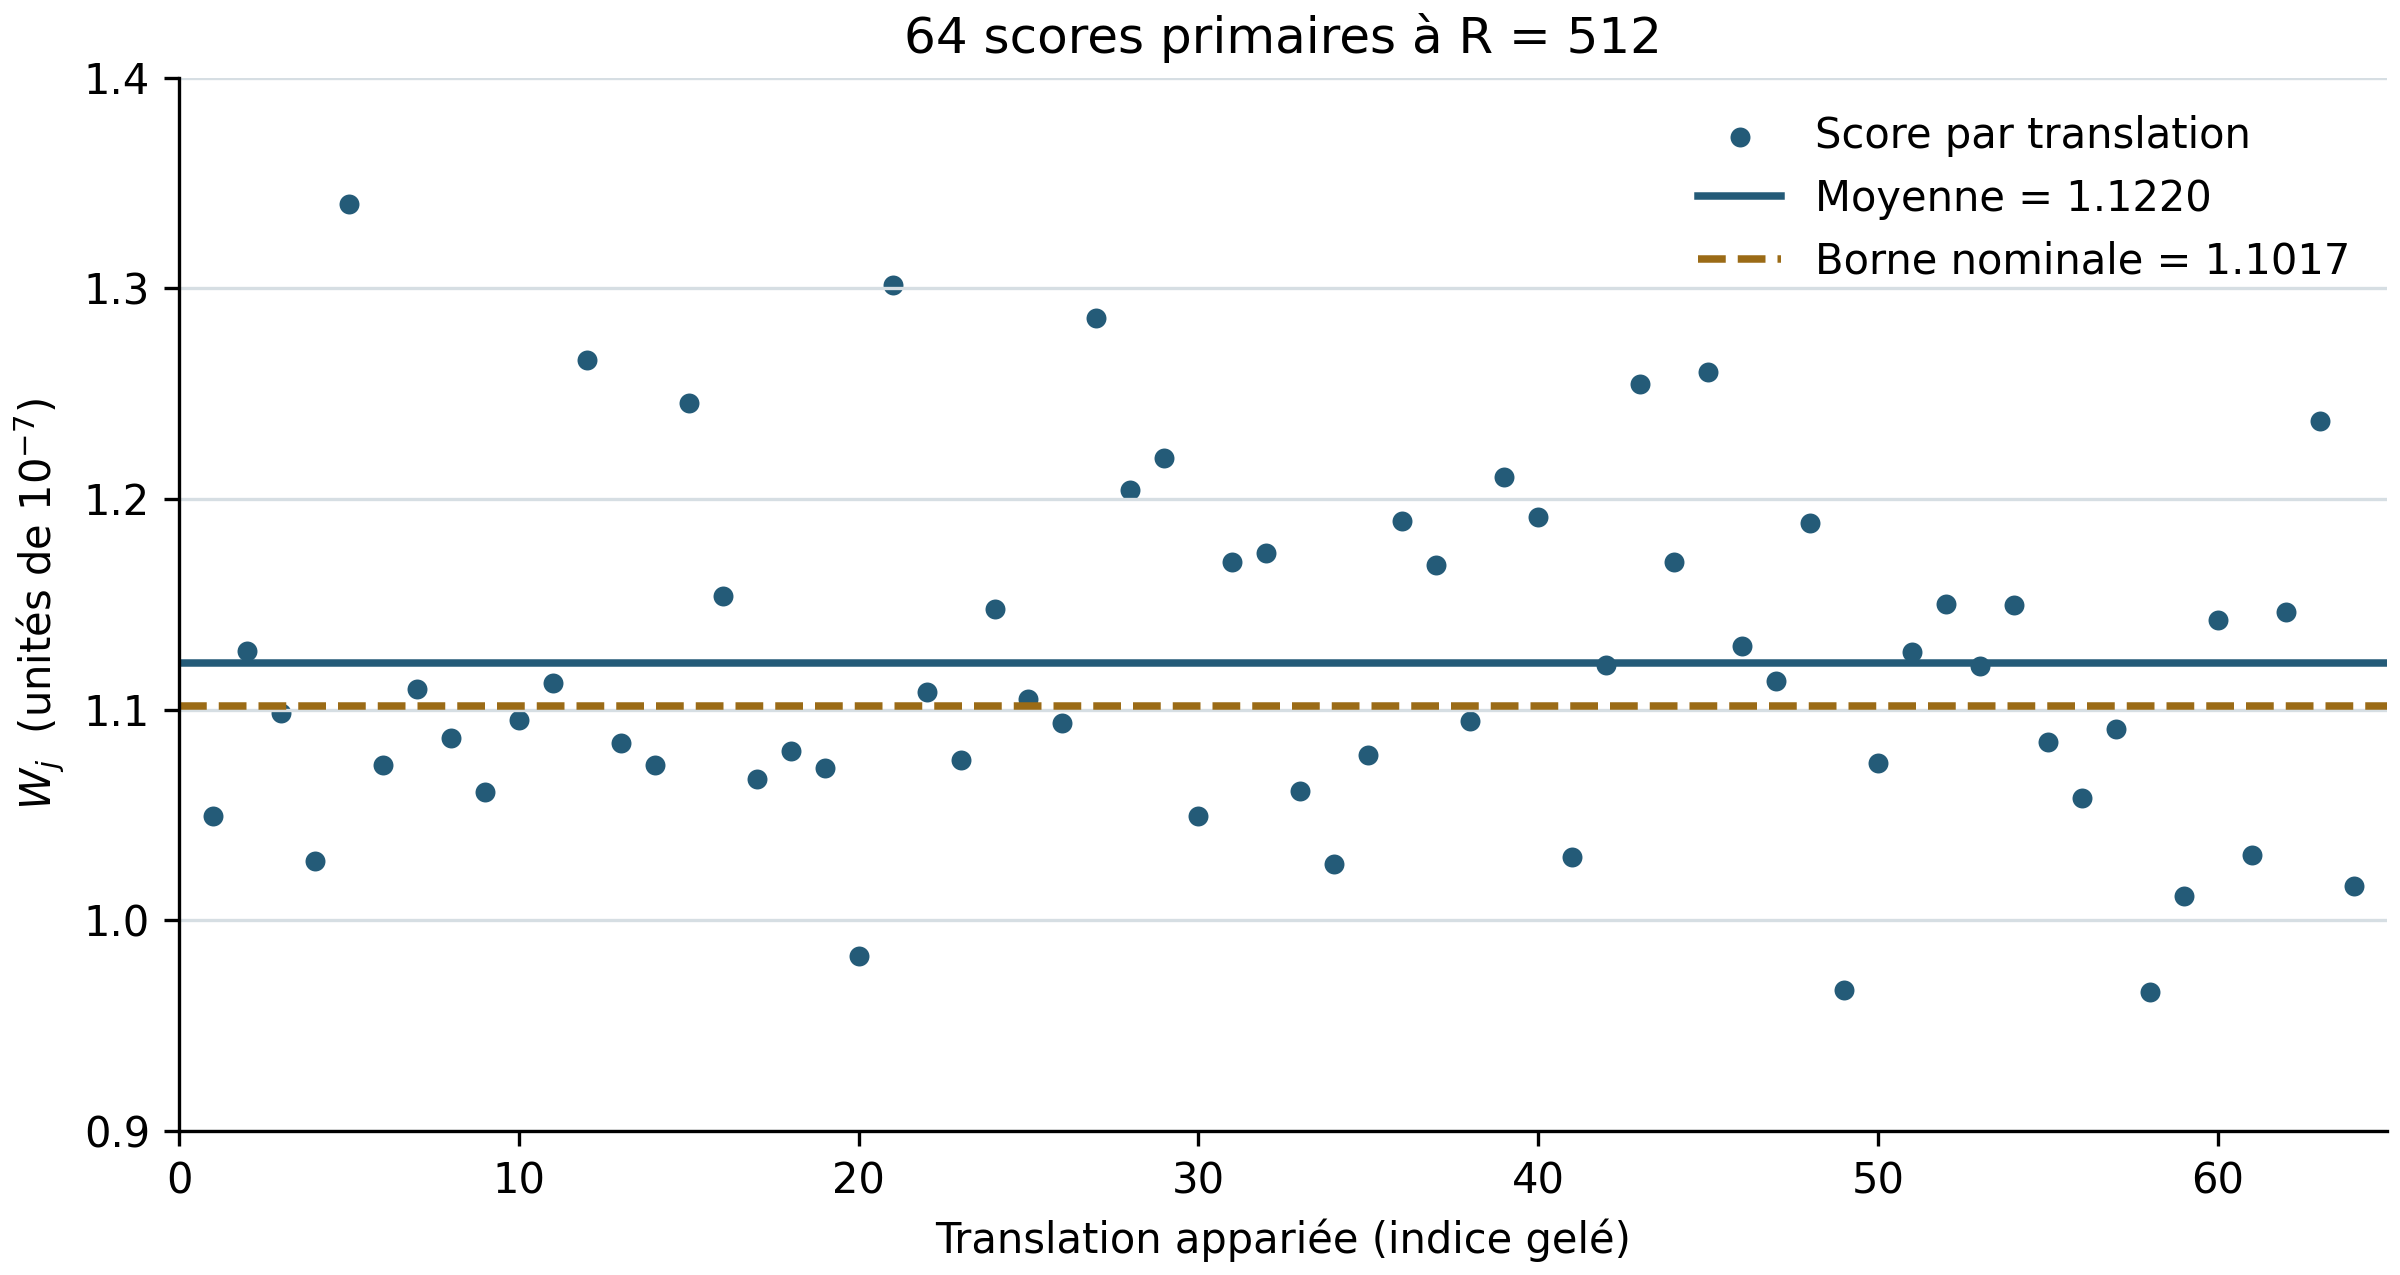
\includegraphics[width=0.92\linewidth]{primary_scores.png}
  \caption{Scores $W_j$ à $R=512$. La ligne bleue indique la moyenne et la ligne pointillée la borne inférieure de Student unilatérale nominale à $97{,}5\,\%$. Unités : $10^{-7}$.}
  \label{fig:primaryscores}
\end{figure}

\section{Résultats secondaires}

\subsection{Profil des sept exposants}

\begin{table}[htbp]
\centering
\caption{Perte moyenne sur $a_3$ : moyenne égale des neuf cellules par translation, puis moyenne sur 64 translations.}
\label{tab:betagrid}
\begin{tabular}{@{}ccc@{}}
\toprule
$\beta$ & $R=256$ & $R=512$ \\
\midrule
$0{,}30$ & $9{,}3735918971\times10^{-7}$ & $3{,}4914111507\times10^{-7}$ \\
$0{,}31$ & $4{,}9180717326\times10^{-7}$ & $1{,}3584206862\times10^{-7}$ \\
$0{,}32$ & $2{,}0665957697\times10^{-7}$ & $\mathbf{7{,}9436733605\times10^{-8}}$ \\
$1/3$   & $\mathbf{6{,}5329308465\times10^{-8}}$ & $2{,}3777428811\times10^{-7}$ \\
$0{,}34$ & $9{,}3084015433\times10^{-8}$ & $4{,}1313395068\times10^{-7}$ \\
$0{,}35$ & $2{,}5298851743\times10^{-7}$ & $7{,}9172227668\times10^{-7}$ \\
$0{,}36$ & $5{,}4994120076\times10^{-7}$ & $1{,}3041549654\times10^{-6}$ \\
\bottomrule
\end{tabular}
\end{table}

Le minimum sur les sept points de grille est $1/3$ à $R=256$ et $0{,}32$ à $R=512$. Aucun optimum continu entre ces points n'est identifié. Le contraste brut apparié $D_{512}-D_{256}$ a pour moyenne
$2{,}996678230058189\times10^{-7}$ et est positif pour les 64 translations. Le rapport des deux pertes moyennes du comparateur affine $\beta=1/3$, $\overline L_{512}/\overline L_{256}$, vaut $3{,}6396265886711663$. Sur ces deux rayons, le raffinement n'entraîne donc pas une amélioration monotone de ce critère ; cette observation ne décide pas le comportement asymptotique.

\subsection{Hétérogénéité d'orientation et de contraction}

La figure~\ref{fig:heterogeneity} montre les moyennes cellulaires brutes et diminuées de $B$. À $R=512$, huit moyennes $D$ sur neuf sont positives, mais six seulement ont une moyenne $D-B$ positive.

\begin{figure}[!htbp]
  \centering
  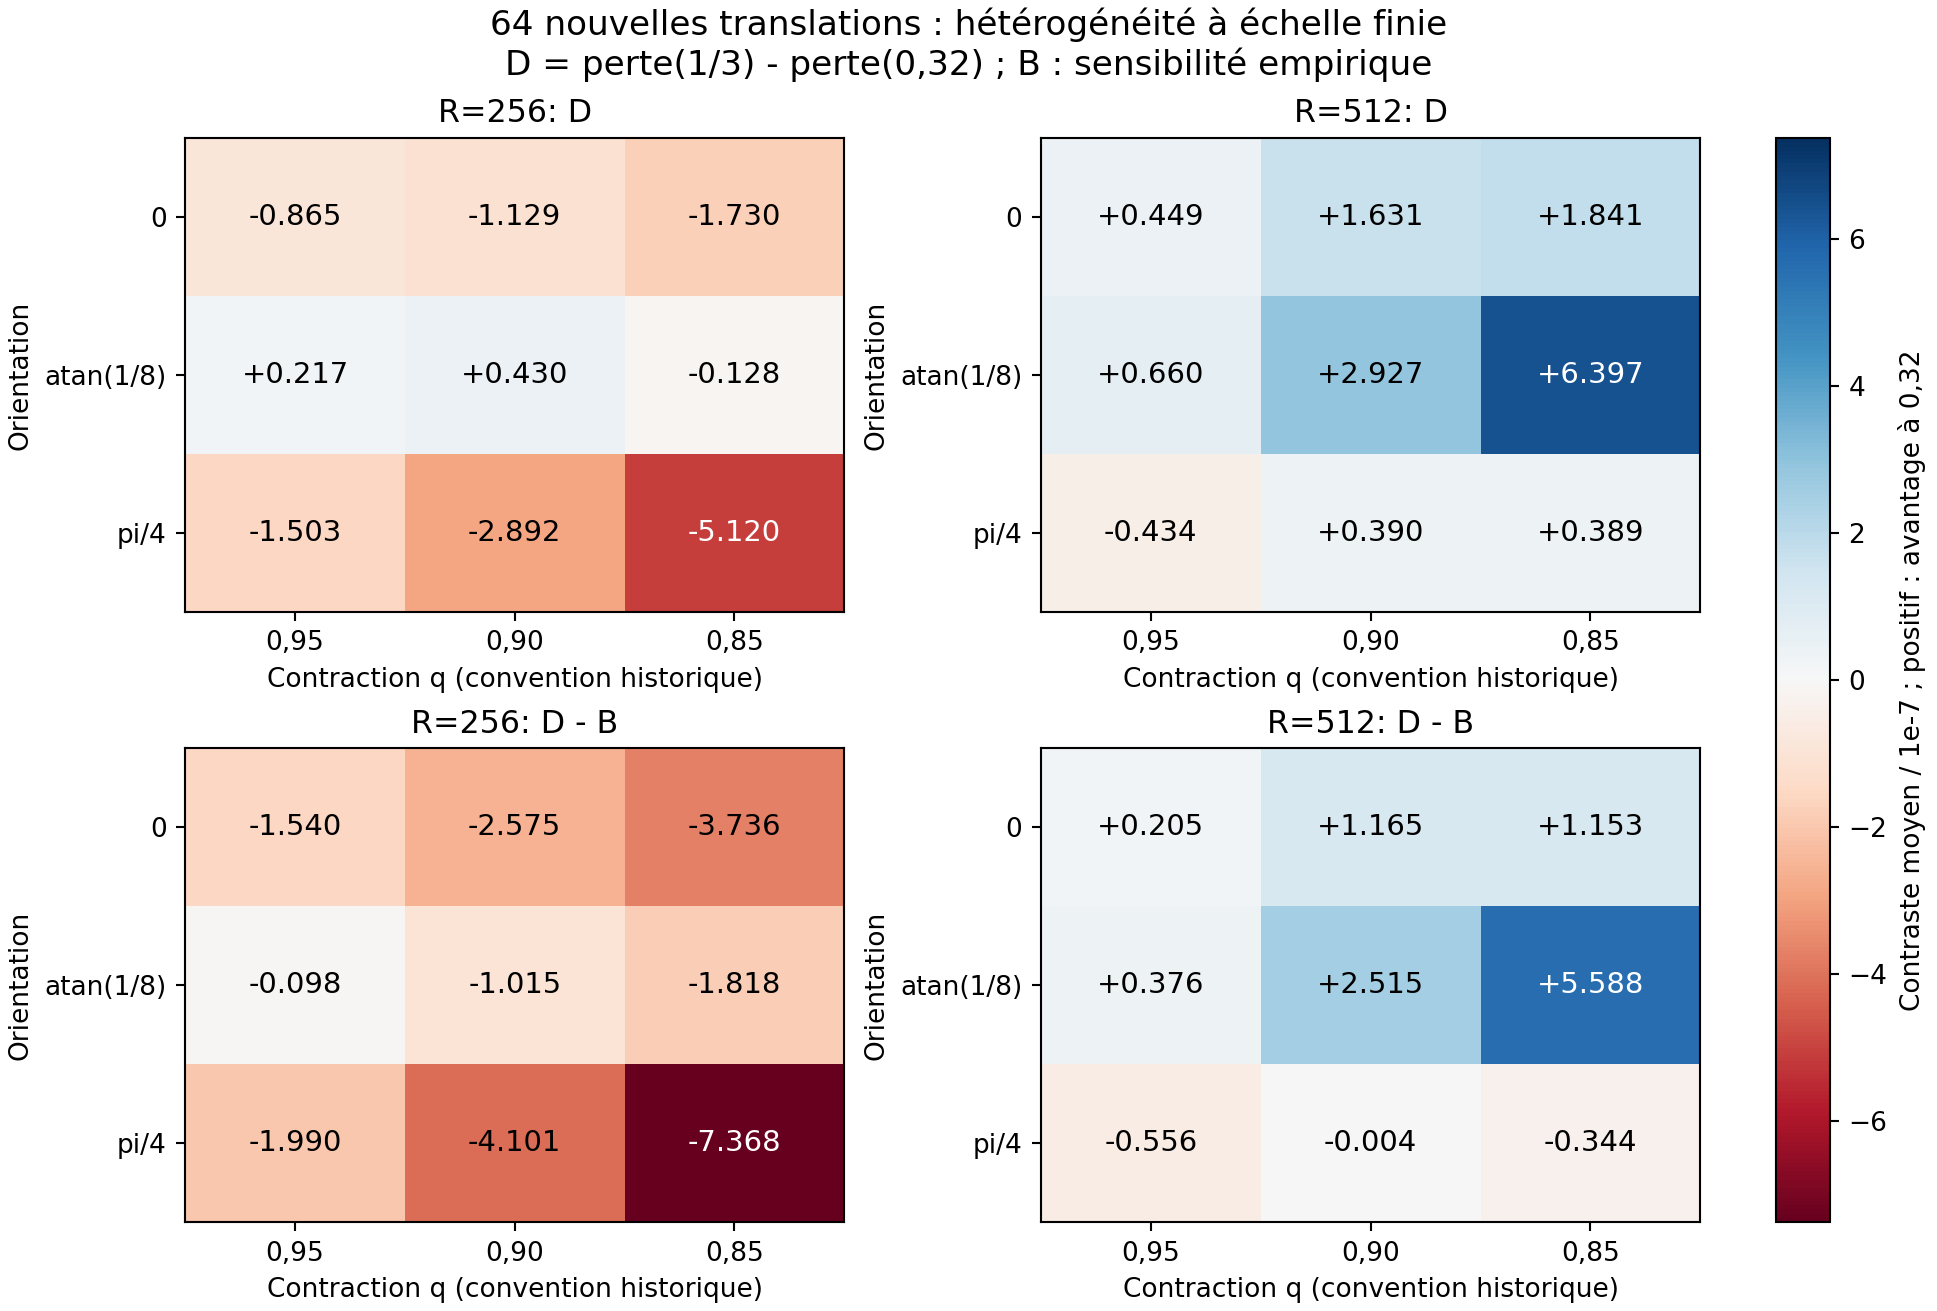
\includegraphics[width=0.96\linewidth]{secondary_contrasts_v05.png}
  \caption{Contrastes moyens sur 64 traductions, en unités de $10^{-7}$. Un contraste brut $D>0$ correspond à une perte plus faible pour $0{,}32$. Une marge $D-B<0$ signifie que l'avantage de $0{,}32$ n'est pas conservé sous la sensibilité soustraite ; elle ne prouve pas, à elle seule, un avantage de $1/3$.}
  \label{fig:heterogeneity}
\end{figure}

\begin{table}[htbp]
\centering
\caption{Cas $R=512$, $\theta=\pi/4$.}
\label{tab:pi4}
\begin{tabular}{@{}cccc@{}}
\toprule
$q$ & moyenne $D$ & moyenne $D-B$ & signe du $D$ brut \\
\midrule
$0{,}95$ & $-4{,}3416397723\times10^{-8}$ & $-5{,}5642722163\times10^{-8}$ & $64/64$ négatifs \\
$0{,}90$ & $\phantom{-}3{,}8977934382\times10^{-8}$ & $-3{,}7166768952\times10^{-10}$ & $64/64$ positifs \\
$0{,}85$ & $\phantom{-}3{,}8878364808\times10^{-8}$ & $-3{,}4356916474\times10^{-8}$ & $60/64$ positifs \\
\bottomrule
\end{tabular}
\end{table}

En particulier, la cellule $q=0{,}95$ favorise $1/3$ pour les 64 translations. La préférence moyenne pour $0{,}32$ n'est donc pas uniforme. Un contrôle descriptif calculé après le résultat primaire donne aussi $D+B<0$ sur les 64 lignes de cette cellule, avec une moyenne $-3{,}1190073284\times10^{-8}$. Ce diagnostic utilise le même budget empirique ; il n'est pas présenté comme un second test confirmatoire. L'expression « résonance diagonale » peut servir d'hypothèse descriptive, mais aucune cause de ce type n'est démontrée ici.

\section{Contrôles et reproductibilité}

\subsection{Recomposition statistique}

Un vérificateur portable, distinct de l'analyseur gelé, lit le CSV sauvegardé et recompose les pertes, les quatre composantes de $B$, les 1\,152 contrastes et les 64 scores. Deux recompositions locales ont retrouvé exactement les champs de contraste et les statistiques primaires, à l'arrondi flottant près. Les 8\,064 clés scientifiques sont uniques ; aucune valeur non finie ni sensibilité négative n'a été détectée. Les 64 coordonnées sont dyadiques, distinctes et sans intersection avec les 48 paires historiques.

Cette recomposition vérifie l'arithmétique statistique à partir des données sauvegardées ; elle ne valide ni la construction géométrique, ni l'oracle continu, ni la chronologie de collecte.

\subsection{Polygones sauvegardés et contrôle géométrique}

L'archive de production contient les 64 fichiers géométriques principaux. Les contrôles v0.6 rapportent la reconstruction des 1\,152 coefficients interpolés $a_3$ depuis ces polygones, avec un écart maximal au CSV de $7{,}62\times10^{-17}$. Un contrôle géométrique détaillé porte sur les huit lignes prescrites et $30\,863$ couches : intervalles entiers, retrait des seuls sommets, comptes, convexité stricte, imbrication, périmètres et empreintes ont été vérifiés. L'intégration de Fourier indépendante présente des écarts maximaux de $3{,}26\times10^{-16}$ aux extrémités et $2{,}98\times10^{-16}$ après interpolation.

Ce contrôle est exhaustif couche par couche sur les huit lignes prescrites seulement ; il ne couvre pas les 64 trajectoires. QuickHull fournit une implémentation partiellement indépendante du calcul des enveloppes et des retraits, mais partage des primitives et les lignes initiales qualifiées avec le moteur principal ; ses polygones n'ont pas été sauvegardés séparément.

\subsection{Dépendances gelées retrouvées}

Les quatre dépendances externes au petit dossier de transmission ont été retrouvées dans le projet d'origine avec les empreintes annoncées :
\begin{itemize}
  \item \code{support\_shape\_engine.py}\\[-0.2em]
    \sha{f1769af06d914f5ff078a3c22c5c259b8777656d5c3596321362766a6e51a191};\par
  \item \code{baseline/polygon\_fourier.py}\\[-0.2em]
    \sha{ec5bcec9b6e5c52bc136f39ee9c27a82a2fbc7c03b2493b24de321c3b4446245};\par
  \item \code{targeted\_supports.npz}\\[-0.2em]
    \sha{5efc10d213e334b0a09d8686b4f7aa3f4f6950d6735a96cbba6999165517530e};\par
  \item \code{extension\_supports.npz}\\[-0.2em]
    \sha{36de3f31f8fdd3c2f02e680a18433f272623c9abfbbf6aeac8452307d69e3ea4}.\par
\end{itemize}
Le paquet public en conserve des copies identifiées et des chemins relatifs. Cela améliore l'autonomie documentaire, mais les scripts historiques gardent leur provenance et leurs anciens chemins ; le mode portable fourni est centré sur la recomposition des statistiques. Aucune nouvelle campagne n'est nécessaire pour vérifier les résultats rapportés.

\section{Limites et portée scientifique}

La portée de l'expérience est volontairement restreinte : une forme initiale, deux rayons, trois orientations, trois contractions et une perte sur le seul coefficient $a_3$. Les 64 traductions appariées fournissent le grain de l'inférence ; les cellules et les sept valeurs de $\beta$ ne sont pas des réplications supplémentaires.

Les réserves principales sont les suivantes :
\begin{itemize}
  \item la borne de Student est nominale et sa couverture est approchée ;
  \item les budgets numériques sont empiriques et non certifiés par intervalles ;
  \item la sélection de $0{,}32$ vient de l'exploration, puis le contraste a été testé sur de nouvelles translations ;
  \item deux rayons ne permettent ni extrapolation asymptotique ni estimation d'un exposant exact ;
  \item l'hétérogénéité observée interdit une formulation uniforme en orientation ou en contraction ;
  \item la nouveauté bibliographique précise n'a pas fait l'objet d'une revue exhaustive ;
  \item aucune relecture scientifique humaine indépendante n'est attestée à la date de cette version.
\end{itemize}

Cette note ne propose aucune nouvelle valeur de $\pi$, aucun théorème de convergence, aucune réfutation asymptotique du flot affine, et aucune validation physique ou générale de la Dynagénèse.

\section{Assistance par intelligence artificielle et relecture sollicitée}

Le protocole, le code, les contrôles et la rédaction ont été élaborés dans un flux assisté par intelligence artificielle sous la responsabilité de l'auteur. Pour la version publique, Codex a inventorié les sources, recomposé les statistiques depuis le CSV sauvegardé, vérifié les empreintes et les dépendances, préparé la source LaTeX, contrôlé le rendu PDF et assemblé les métadonnées de diffusion. Les systèmes d'IA ne sont pas listés comme auteurs et ne remplacent pas une expertise scientifique humaine.

Une relecture spécialisée est sollicitée, en priorité sur la comparabilité géométrique à périmètre égal, le budget de sensibilité de l'équation~\eqref{eq:B}, l'interprétation du basculement entre $R=256$ et $R=512$, et les limites de l'inférence au-delà du cadre observé.

\section{Disponibilité des données, du code et des archives}

Le dépôt public \href{\repo}{\repo} contient la source éditable, le PDF, les figures, les données compactes, le vérificateur portable, les sources gelées permises, les dépendances retrouvées, les contrôles v0.6 et un manifeste SHA-256. La version archivée sur Zenodo est identifiée par \href{https://doi.org/\versiondoi}{\versiondoi}.

L'archive de production après collecte, exclue de l'historique Git en raison de sa taille, est fournie comme supplément de release et sur Zenodo :
\begin{center}
\small
\code{\_prepare\_replication\_v0\_4\_20261027.zip}\\
SHA-256 : \sha{f225c317be686798471e52a2f34e2bbc2fdf22406654702aeebf197797764dc3}.
\end{center}
L'archive d'exécution a pour SHA-256 :
\begin{center}
\sha{a883fcd2776a4f3b70e0992a5312c4a2a49cf4860dfa483f35539c50e0c32378}.
\end{center}

\section{Conclusion}

Le critère prospectif gelé est satisfait : à $R=512$, le score moyen apparié après soustraction de la sensibilité empirique favorise $\beta=0{,}32$ face à $1/3$ sur les 64 nouvelles translations. Ce résultat fini est robuste aux retraits-un-par-un au niveau du score agrégé. Il coexiste avec un classement inversé à $R=256$ et avec des cellules défavorables, notamment $\theta=\pi/4$, $q=0{,}95$. La conclusion appropriée est donc une préférence moyenne, locale au plan observé, et non une loi universelle.

\bibliographystyle{plainnat}
\bibliography{references}

\appendix
\section{Niveaux de vérification à ne pas confondre}

\begin{table}[htbp]
\centering
\caption{Portée des contrôles disponibles.}
\begin{tabularx}{\linewidth}{@{}>{\raggedright\arraybackslash}p{0.25\linewidth}X@{}}
\toprule
Niveau & Ce qui est vérifié, et limite correspondante \\
\midrule
Recomposition statistique & Calculs depuis les 8\,064 lignes sauvegardées ; ne reconstruit pas les couches ni l'oracle. \\
Polygones sauvegardés & Reconstruction des 1\,152 coefficients interpolés depuis les 64 fichiers géométriques principaux. \\
Contrôle géométrique détaillé & Huit lignes et 30\,863 couches ; ne couvre pas intégralement 64 trajectoires. \\
Moteur QuickHull & Contrôle partiellement indépendant ; partage des primitives et les lignes initiales qualifiées. \\
Relecture humaine & Sollicitée, mais non effectuée pour la version 0.1. \\
\bottomrule
\end{tabularx}
\end{table}

\section{Empreintes structurantes}

\begin{tabularx}{\linewidth}{@{}p{0.36\linewidth}X@{}}
\toprule
Objet & SHA-256 \\
\midrule
Manifeste gelé précollecte & \sha{023b69c57501ed27ccba892b0e2c2afee88fa1621f711d6c057e3dc0a58f2518} \\
Archive de production v0.4 & \sha{f225c317be686798471e52a2f34e2bbc2fdf22406654702aeebf197797764dc3} \\
Archive d'exécution v0.5 & \sha{a883fcd2776a4f3b70e0992a5312c4a2a49cf4860dfa483f35539c50e0c32378} \\
CSV de campagne & \sha{7f998f71c897eb1f9e1541f593a2600e56a34233f90661990dfcafd17c2f286e} \\
\bottomrule
\end{tabularx}

\end{document}
